\section{Discrete Random Variables}
\emph{Motivation}: Roll two dice.
$\Omega = \{1, \dots, 6\}^2 = \{(i, j) : 1 \leq i, j \leq 6\}.$
If we restrict our attention to:
\begin{itemize}
    \item the first dice e.g. $\{(i, j) : i = 3\}$.
    \item the sum of the dice e.g. $\{(i, j) : i + j = 8\}$.
    \item the max of the dice e.g. $\{(i, j) : i, j \leq 4, i \text{ or } j = 4\}$.
\end{itemize} 
This is annoying and we want to move on from sets.

\emph{Goal}: ``Random real-valued measurements'', we want the value of the first dice to be $X$ and the sum to be $X + Y$ \dots

\begin{definition}[Discrete Random Variable]
    A \vocab{discrete random variable} $X$ on a probability space $(\Omega, \mathcal{F}, \mathbb{P})$ is a function $X : \Omega \to \mathbb{R}$ \color{blue} s.t. 
    \begin{itemize}
        \item $\{ \omega \in \Omega : X(\omega) = x\} \in \mathcal{F}$
        \item $\operatorname{Image}(X)$ if finite or countable (subset of $\mathbb{R}$).
    \end{itemize}
    \color{red} 
    \begin{itemize}
        \item We abbreviate $\{ \omega \in \Omega : X(\omega) = x\}$ as $\{X = x\}$. So $\mathbb{P}(X = x)$ is valid.
        \item Often $\operatorname{Image}(X) = \mathbb{Z}$ or $\mathbb{N}_0$ or $\{0, 1\}$ etc. \emph{not} $\{\text{Heads or Tails}\}$. 
    \end{itemize} \color{black}
    If $\Omega$ is finite or countable and $\mathcal{F} = \mathcal{P}(\Omega)$ both blue bullet points hold automatically.
\end{definition} 

\begin{example}[Part II Applied Probability] \mbox{}
    {\par \centering 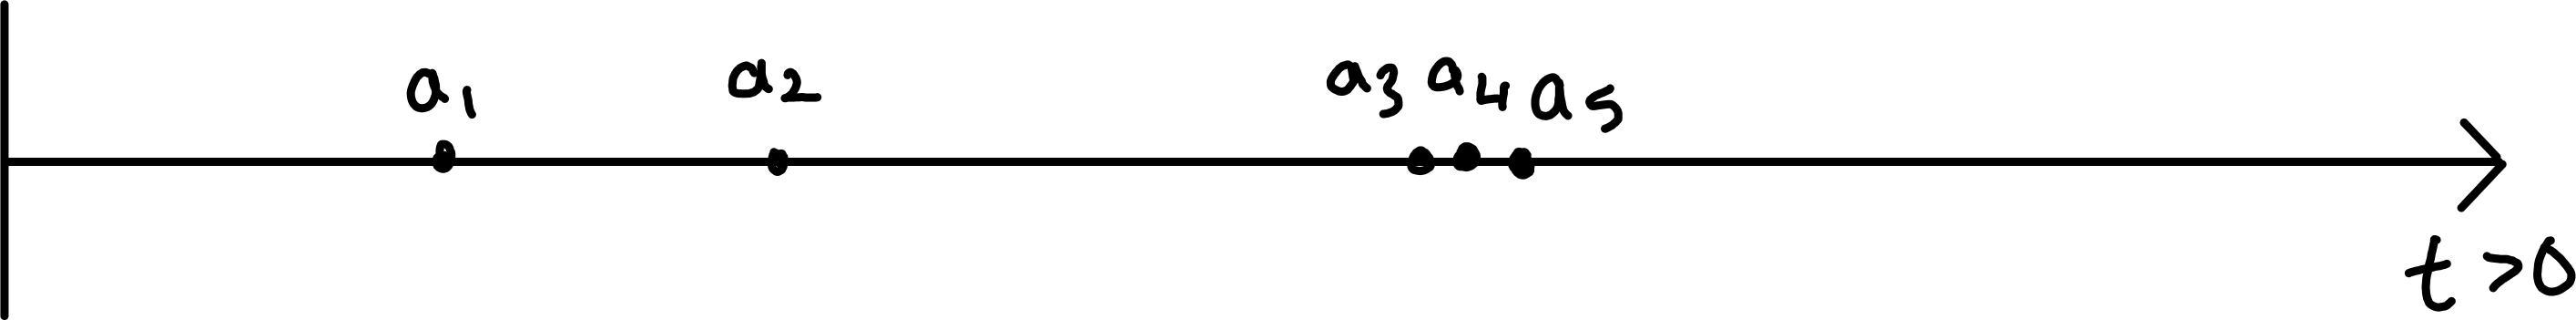
\includegraphics[height=5cm]{04-queue} \par}
    ``random arrival process''.
    Let $\Omega = \{\text{countable subsets } (a_1, a_2, \dots) \text{ of } (0, \infty)\}$ and $N_t =$ number of arrivals by time $t = |\{a_i : a_i \leq t\}| \in \mathbb{N}_0$ is a discrete RV (random variable) for each time $t$.
\end{example} 

\begin{definition}[Probability Mass Function]
    The \vocab{probability mass function} of discrete RV $X$ is the function $p_X : \mathbb{R} \to [0, 1]$ given by $p_X(x) = \mathbb{P}(X = x) \quad \forall \; x \in \mathbb{R}$.
\end{definition} 

\begin{note} \mbox{}
    \begin{itemize}
        \item if $x \notin \operatorname{Image}(X)$ then $p_X(x) = \mathbb{P}(\{\omega \in \Omega : X(\omega) = x\}) = \mathbb{P}(\emptyset) = 0$.
        \item \begin{align*}
            \sum_{x \in \operatorname{Im}(X)} p_X(x) &= \sum_{x \in \operatorname{Im}(X)} \mathbb{P}(\underbracket{\{\omega \in \Omega : X(\omega) = x\}}_{\color{blue} \text{disjoint}}) \\
            &= \mathbb{P}\left(\bigcup_{x \in \operatorname{Im}(X)} \{\omega \in \Omega : X(\omega) = x\} \right) \\
            &= \mathbb{P}(\Omega) \\
            &= 1
        \end{align*} 
    \end{itemize} 
\end{note} 
 
\begin{example}[Indicator function]
    For event $A \in \mathcal{F}$, define $1_A : \Omega \to \mathbb{R}$ by 
    \begin{align*}
        1_A(\omega) &= \begin{cases}
            1 & \text{if } \omega \in A \\
            0 & \text{else }
        \end{cases}  
    \end{align*} 
    $1_A$ is a discrete RV with $\operatorname{Image} = \{0, 1\}$.
    $p_{1_A}(1) = \mathbb{P}(1_A = 1) = \mathbb{P}(A)$, $p_{1_A}(0) = \mathbb{P}(1_A = 0) = \mathbb{P}(A^c)$ and $p_{1_A}(x) = 0 \quad \forall \; x \notin \{0, 1\}$.

    \color{blue} This encodes ``did $A$ happen'' as a real number.
\end{example} 

\begin{remark}
    Given a pmf $p_X$ (probability mass function), we can always construct a probability space $(\Omega, \mathcal{F}, \mathbb{P})$ and a RV defined on it with this pmf.

    \color{blue}
    \begin{itemize}
        \item $\Omega = \operatorname{Im}(X)$ i.e. $\{x \in \mathbb{R} : p_X(x) > 0\}$
        \item $\mathcal{F} = \mathcal{P}(\Omega)$
        \item $\mathbb{P}(\{x\}) = p_X(x)$ and extend to all $A \in \mathcal{F}$
    \end{itemize} 
\end{remark} 

\subsection{Discrete Probability Distributions}
$\Omega$ is finite.

\subsubsection{Bernoulli distribution - ``(biased) coin toss"}

If $X \sim \operatorname{Bern}(p)$ where $p \in [0, 1]$ then $\operatorname{Im}(X) = \{0, 1\}$ and $p_X(1) = \mathbb{P}(X = 1) = p$ and $p_X(0) = 1 - p$.

\begin{example}
    $1_A \sim \operatorname{Bern}(p)$ with $p = \mathbb{P}(A)$.
\end{example} 

\subsubsection{Binomial distribution}
This can be used to model the number of heads when a coin is tossed $n$ times.

If $X \sim \operatorname{Bin}(n, p)$ where $n \in \mathbb{Z}^+$ and $p \in [0, 1]$ then $\operatorname{Im}(X) = \{0, 1, \dots, n\}$, $p_X(k) = \mathbb{P}(X = k) = \binom{n}{k} p^k (1- p)^{n -k}$.
$\sum_{k=0}^{n} p_X(k) = (p + (1-p))^n = 1$.

\subsubsection{More than one RV}

\emph{Motivation}: Roll a dice with outcome $X \in \{1, 2, \dots, 6\}$.
Events: $A = \{1 \text{ or } 2\}$, $B = \{1 \text{ or } 2 \text{ or } 3\}$, $B = \{1 \text{ or } 3 \text{ or } 5\}$.
$1_A \sim \operatorname{Bern}\left(\frac{1}{3}\right)$, $1_B \sim \operatorname{Bern}\left(\frac{1}{2}\right)$, $1_C \sim \operatorname{Bern}\left(\frac{1}{2}\right)$.\\
\emph{Note}: $1_A \leq 1_B$ for all outcomes \\
but $1_A \leq 1_C$ for all outcomes \emph{is false}.

\begin{definition}[Independent RVs]
    Let $X_1, \dots, X_n$ be discrete RVs.
    We say $X_1, \dots, X_n$ are \emph{independent} if:
    \begin{align*}
        \mathbb{P}(X_1 = x_1, \dots, X_n = x_n) &= \mathbb{P}(X_1 = x) \dots \mathbb{P}(X_n = x_n) \quad \forall \; x_1, \dots, x_n \in \mathbb{R}.
    \end{align*} 
    \color{blue} (suffices to check $\forall \; x_i \in \operatorname{Im}(X_i)$)
\end{definition} 

\begin{example}
    $X_1, \dots, X_n$ independent RVs each with the Bernoulli(p) distribution.
    Study $S_n = X_1 + \dots + X_n$.
    Then 
    \begin{align*}
        \mathbb{P}(S_n = k) &= \sum_{\substack{x_1 + \dots + x_n = k \\ x_i \in \{0, 1\} }}\mathbb{P}(X_1 = x_1, \dots, X_n = x_n) \\
        &= \sum_{x_1 + \dots + x_n = k} \mathbb{P}(X_1 = x_1) \dots \mathbb{P}(X_n = x_n) \\
        &= \sum_{x_1 + \dots + x_n = k} p^{|\{i : x_i = 1\}|} (1 - p)^{|\{i : x_i = 0\}|} \\
        &= \sum_{x_1 + \dots + x_n = k} p^k (1-p)^{n - k} \\
        &= \binom{n}{k} p^k (1-p)^{n - k}.
    \end{align*} 
    So $S_n \sim \operatorname{Bin}(n, p)$.
\end{example} 

\begin{example}[Non-example]
    $(\sigma(1), \sigma(2), \dots, \sigma(n))$ a uniform permutation.
    \begin{claim}
        $\sigma(1)$ and $\sigma(2)$ are \emph{not} independent.
    \end{claim} 
    Suffices to find $i_1, i_2$ s.t. $\mathbb{P}(\sigma(1) = i_1, \sigma(2) = i_2) \neq \mathbb{P}(\sigma(1) = i_1) \mathbb{P}(\sigma(2) = i_2)$.
    E.g. $\mathbb{P}(\sigma(1) = 1, \sigma(2) = 1) = 0 \neq \underbracket{\mathbb{P}(\sigma(1) = 1) \mathbb{P}(\sigma(2) = 1)}_{= 1 / n \times 1 /n}$
\end{example} 

Consequence of definition

Let $X_1, \dots, X_n$ be independent.
Then $\mathbb{P}(X_1 \in A_1, \dots, X_n \in A_n) = \mathbb{P}(X \in A_1) \dots \mathbb{P}(X_n \in A_n) \quad \forall \; A_1, \dots, A_n \subset \mathbb{R}$ countable.

Let $\Omega = \mathbb{N}$, "Ways of choosing a random integer"

\subsubsection{Geometric distribution (``Waiting for success'')}
This can be used to model the number of coin tosses until we get a head.

If $X \sim \operatorname{Geo}(p)$ were $p \in (0, 1)$.
$\operatorname{Im}(X) = \{1, 2, \dots\}$, \\
$p_X(k) = \mathbb{P}(\text{(k-1) failures, then success on the kth trial}) = (1-p)^{k-1}p$.
\color{blue} Check: $\mathcolor{blue}{\sum_{k \geq 1} (1-p)^{k - 1} p = p \sum_{t \geq 0} (1-p)^t = \frac{p}{1 - (1 - p)} = 1}$.\color{black}

Alternatively: ``Count how many failures before a success'' \\
$\operatorname{Im}(Y) = \{0, 1, 2, \dots\}$, $p_Y(k) = \mathbb{P}(\text{k failures, then success on the (k+1)th trial})$.
\color{blue} Check: $\mathcolor{blue}{\sum_{k \geq 0} (1-p)^{k} p = 1}$.\color{black}

\subsubsection{Poisson Distribution}
If $X \sim \operatorname{Po}(\lambda)$ (or $\operatorname{Poi}(\lambda)$) with $\lambda \in (0, \infty)$.
$\operatorname{Im}(X) = \{0, 1, 2, \dots\}$ and $\mathbb{P}(X = k) = e^{- \lambda} \lambda^k / k! \quad \forall \; k \geq 0$.
\color{blue} Check: $\mathcolor{blue}{\sum_{k \geq 0} \mathbb{P}(X = k) = e^{^\lambda} \sum_{k \geq 0} \frac{\lambda^k}{k!} = e^{\lambda} e^\lambda}$.\color{black}

\text{Motivation}: Consider $X_n \sim \operatorname{Bin}(n, \frac{\lambda}{n})$
    \begin{example}[``Arrival proccess'']
    {\par \centering 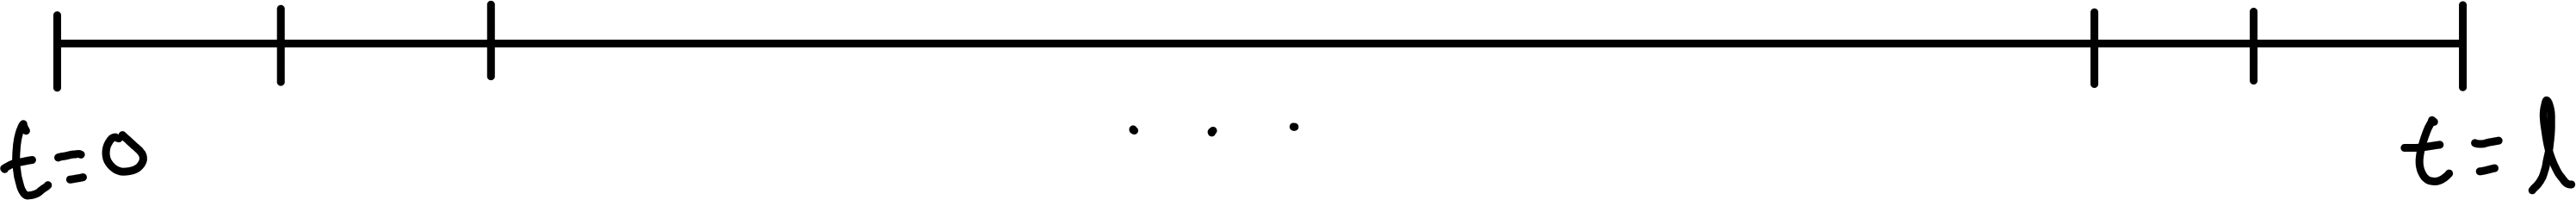
\includegraphics[height=5cm]{04-arrival} \par}
    \begin{itemize}
        \item Split time interval $[0, \lambda]$ into $n$ small intervals.
        \item Probability of an arrival in each interval is $p$, independently across intervals.
        \item Total no. of arrivals is $X_n$.
    \end{itemize} 

    \begin{align*}
        \mathbb{P}(X_n = k) &= \binom{n}{k} \left(\frac{\lambda}{n}\right)^k \left(1 - \frac{\lambda}{n}\right)^{n - k} \\
        \intertext{\color{blue} Fix $k$ and let $n \to \infty$}
        &= \frac{n!}{n^k (n - k)!} \times \underbracket{\frac{\lambda^k}{k!}}_{\text{no n}} \times \underbracket{\left(1 - \frac{\lambda}{n}\right)^n}_{\to e^{-\lambda}} \times \underbracket{\left(1 - \frac{1}{n}\right)^{-k}}_{\to 1} \\
        \frac{n!}{n^k (n - k)!} &= \frac{n (n-1) \dots (n - k + 1)}{n^k} \\
        &= 1 \times \left(1 - \frac{1}{n}\right) \times \left(1 - \frac{2}{n}\right) \times \dots \times \left(1 - \frac{k - 1}{n}\right) \\
        &\to 1 \quad \text{There are a fixed number of terms all converging to 1} \\
        \mathbb{P}(X_n = k) &\underset{n \to \infty}{\to} e^{-\lambda} \frac{\lambda^k}{k!}.
    \end{align*} 
\end{example} 